\vspace{-10pt}
\section{Related Work}

\subsection{Object Goal Navigation}
Object Goal Navigation (ObjectNav)~\cite{batra2020objectnav} is a semantic target-driven task where agents navigate to specified object categories in unknown environments based on egocentric observations.
While early methods require task-specific training (e.g., reinforcement learning~\cite{ye2021auxiliary,chang2020semantic,deitke2022procthor,gireesh2022object}, imitation learning~\cite{ramrakhya2023pirlnav}) for closed-set object categories, recent zero-shot approaches enable generalization to open-set categories by leveraging foundation models in two main ways.
LLM-based approaches use language models for commonsense reasoning. For instance, L3MVN~\cite{yu2023l3mvn} evaluates frontiers by reasoning about object relationships, while ESC~\cite{zhou2023esc} models room-object knowledge as soft logic constraints. 
VLM-based approaches, in contrast, directly extract semantic information from visual observations. For example, VLFM~\cite{yokoyama2024vlfm} constructs language-grounded value maps using cosine similarity scores. More recently, ApexNav~\cite{zhang2025apexnav} adaptively switches between semantic and geometric exploration while maintaining target-centric memory to reduce false detections.
However, existing works predominantly focus on small-scale, semantically homogeneous 2D indoor environments, where structured layouts and semantic hierarchies provide strong cues for object localization. In contrast, our approach extends this task to drone platforms operating in large-scale outdoor scenarios such as urban areas, forests, and waterfront areas. This extension introduces fundamental challenges including extended search ranges, sparse target distribution across unstructured terrain, and the lack of hierarchical semantic organization that indoor methods rely upon. 
% \sysname addresses these challenges through innovations in both system architecture and algorithmic design.
\begin{figure*}[t]
    \centering
    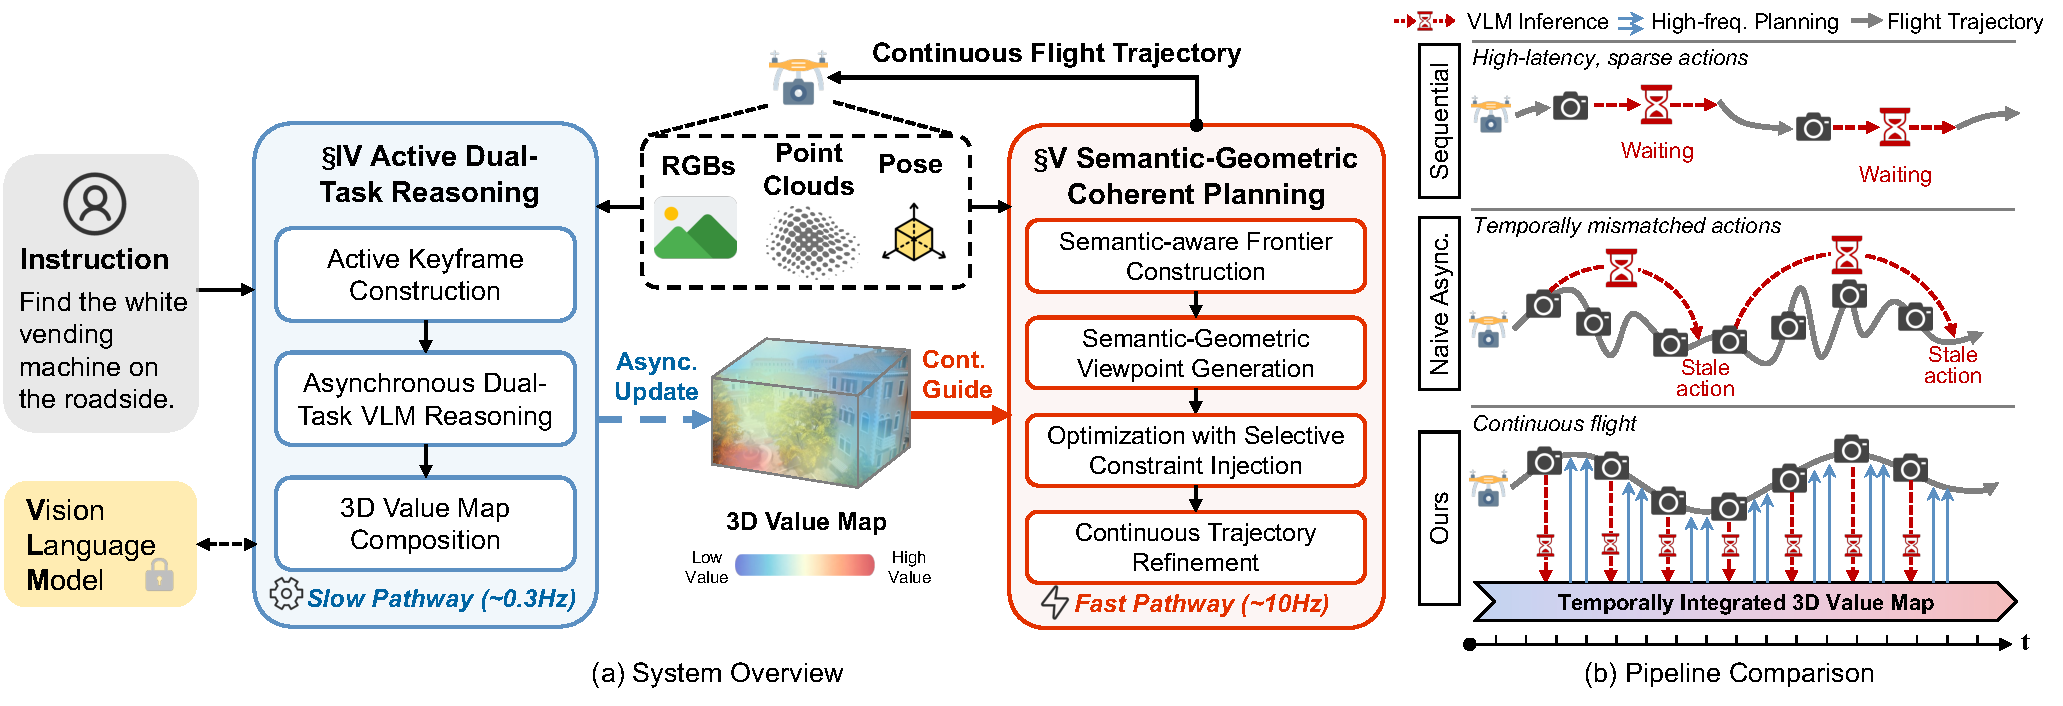
\includegraphics[width=0.99\linewidth]{figures/overview-7.pdf}
    \setlength{\abovecaptionskip}{-18pt}  
    \caption{\textbf{System overview and pipeline comparison.}
    (a) \sysname features a dual-pathway asynchronous architecture. The VLM-driven reasoning pathway extracts language-conditioned semantic priors to update a 3D value map asynchronously (Async.), while the high-frequency planning pathway continuously (Cont.) harvests this evolving semantic memory to generate motion trajectories. This design enables both modules to operate at their native frequencies while achieving effective synergy, eliminating mutual blocking.
    (b) Pipeline Comparison. The Sequential approach requires drones to hover for VLM responses, leading to fragmented flight and low search efficiency. The Naive Asynchronous approach enables movement during VLM inference but suffers from action mismatch, as action commands are generated based on stale observations. In contrast, \sysname repositions the VLM as a high-level semantic generator and temporally integrates semantic information into a persistent 3D value map, enabling continuous flight with adaptive semantic guidance.
    }
    \label{fig:sysoverview}
    \vspace{-12pt}
\end{figure*}
\subsection{Aerial Object Search}
In recent years, aerial object search has attracted increasing attention, encompassing both geometric-driven~\cite{luo2024star} and information-driven~\cite{dang2018autonomous} methods. However, these approaches have predominantly relied on closed-set target detectors. While they excel in structured indoor environments, they cannot leverage rich semantic information in scenes to improve search efficiency, nor can they generalize to open-set object categories.
The advancement of embodied intelligence and large language models has introduced new opportunities for drones to understand natural language instructions and locate objects in large-scale, open-world environments. Existing VLM-based methods follow three main paradigms: (\textit{i}) Motion primitive-based selection~\cite{ji2025towards,xiao2025uav}, where VLMs output discrete navigation commands such as moving forward a specified distance based on visual observations; (\textit{ii}) Coordinate selection~\cite{pardyl2025flysearch}, where VLMs identify target locations by choosing from a set of candidate coordinates overlaid on the observed images; and (\textit{iii}) Coordinate prediction~\cite{hu2025see}, where VLMs directly generate 2D pixel coordinates from observed images, which are then projected into 3D space to guide navigation.
While these paradigms demonstrate efficacy in constrained scenarios, they all suffer from stop-and-infer behaviors and over-reliance on VLM decisions, resulting in limited search efficiency when deployed in expansive outdoor environments. 
In contrast, we propose a dual-pathway asynchronous architecture where VLM inference and path planning are decoupled. The planner prioritizes high-value regions inferred by VLMs while minimizing travel distance, generating continuous and consistent flight trajectories that ensure efficient search.


